\documentclass[12pt,a4paper]{article}
\usepackage[brazilian]{babel}
\usepackage[utf8]{inputenc}
\usepackage[T1]{fontenc}
\usepackage[pdftex]{hyperref}
\usepackage{graphicx}
\usepackage{float}
\setlength{\parindent}{2cm}
\begin{document}
\begin{titlepage}
\begin{center}
\large UNIVERSIDADE FEDERAL DE UBERLANDIA \\
\vspace{6cm}
Relatório sobre FPGA e arquitetura MIPS
\vspace{2cm}
\begin{flushright}
João Paulo de Oliveira\\
11611BCC046\\
Graduando em ciência da computação
\end{flushright}
\vspace{8cm}
Uberlândia\\
2017
\end{center}
\end{titlepage}
\section{FPGA}
	\subsection{História}
\qquad No final da década de 1980, o Naval Surface Warfare Center financiou um experimento de Steve Casselman que desenvolveu um computador para implementar 600.000 portas reprogramáveis. Alguns dos conceitos fundamentais da indústria do FPGA, portões e blocos de lógica são fundados em patentes concedidas a David W. Page e LuVerne R. Peterson em 1985. A Altera (1983) e foi produzido o primeiro dispositivo lógico reprogramável da indústria em 1984 - o EP300 - que apresentou uma janela de quartzo no pacote que permitiu aos usuários brilhar uma lâmpada ultravioleta no dado para apagar as células EPROM que mantinham a configuração do dispositivo.Os co-fundadores de Xilinx (1984), Ross Freeman e Bernard Vonderschmitt, inventaram a primeira matriz comercialmente viável de portas programáveis em campo em 1985 - O XC2064 tinha portas programáveis e interconexões programáveis entre portões, os começos De uma nova tecnologia e mercado. O XC2064 tinha 64 blocos lógicos configuráveis CLBs), com duas tabelas de pesquisa de três entradas (LUTs). Altera e Xilinx continuaram sem concorrentes e cresceram rapidamente de 1985 a meados da década de 1990, quando os concorrentes brotaram, reduzindo a participação de mercado significativa. Em 1993, a Actel (agora Microsemi) estava servindo cerca de 18\% do mercado. Em 2010, Altera (31 por cento), Actel (10 por cento) e Xilinx (36 por cento) juntos representavam aproximadamente 77 por cento do mercado FPGA. 
A década de 1990 foi um período de tempo explosivo para FPGAs, tanto em sofisticação quanto no volume de produção. No início da década de 1990, as FPGAs eram principalmente usadas em telecomunicações e redes. No final da década, os FPGAs encontraram seu caminho em aplicações consumidoras, automotivas e industriais.
\subsection{O que é FPGA?}

\begin{figure}[!htb]
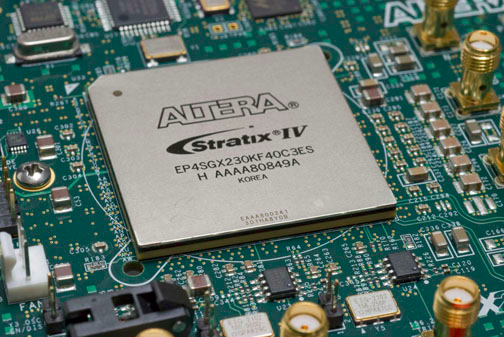
\includegraphics[scale=0.5]{49aWla.png}
\centering 
\caption{Altera Straix IV, Disponível em: $https:// upload.wikimedia.org/ \newline wikipedia/commons/f/fa/Altera_StratixIVGX_FPGA.jpg$}
\end{figure}
\qquad Um FPGA(arranjo de portas programáveis em campo) consistem em um circuito integrado construído de  blocos lógicos, blocos de entrada e saída e chaves de interconexão, porém, esses blocos ser arranjados através de uma linguagem chamada VHDL(Linguagem de descrição de hardware VHSIC), com isso, as saídas podem ser redirecionadas como descrito na linguagem isso faz com que o hardware mude de acordo com a demanda do usuário, como o FPGA é hardware, as operações descritas no código nele carregado são executadas em paralelo, e não sequencialmente como ocorre no software.
	Assim, com o FPGA, torna-se possível “baixar o hardware”, modificá-lo e assim gravar sem nenhuma mudança física, troca de circuitaria. Com ele é possível montar um ou mais processadores, assim eles podem funcionar em paralelo em um único circuito apenas descrevendo na linguagem corretamente, pode ser realizada a engenharia reversa de um programa e implementá-lo no FPGA, além disso, as portas lógicas podem ser conectadas a fim de formar qualquer circuito ou vários circuitos dependendo do número de blocos que essa placa contém.
Nesses circuitos, as funções são implementadas por LUTs (do inglês, look-up tables) que, em sua essência, são tabelas verdade programáveis. Elas podem computar qualquer função booleana de n variáveis, sendo que estas correspondem às entradas da LUT. Assim, a restrição que define a biblioteca virtual é o número de entradas de cada LUT (ou célula lógica). Como o circuito já existe fisicamente, dados como área, atraso e consumo já são previamente conhecidos, restando ao mapeador a tarefa de respeitar restrições de desempenho, minimizando o número necessário de LUTs.
\subsection{Arquitetura}
\begin{figure}[!htb]
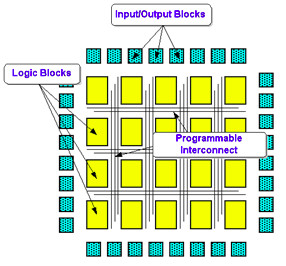
\includegraphics[scale=1]{sistema_fpga.jpg}
\centering
\caption{Esquema de arquitetura do FPGA Disponível em: \newline http://vhdl.com.br/site/fpga/conceitos-basicos}
\end{figure}
\begin{itemize}
\item \textbf{Logical Blocks(CLB):} Circuitos  construídos pela união de flip-flops e lógica combinacional. Utilizando os LBs, um usuário pode construir elementos funcionais lógicos.
\item \textbf{Input/Output Block(IOB):}São basicamente buffers, que funcionam como um pinos bidirecionais de entrada e saída do FPGA.
\item \textbf{Switch Matrix(Programmable Interconnect da figura):} Trilhas utilizadas para conectar os LBs e IOBs, é composto pelas interconexões. Os recursos de interconexões possuem trilhas para conectar as entradas e saídas dos LBs e IOBs para as redes apropriadas. O processo de escolha das interconexões é chamado de roteamento. 
\end{itemize}

\subsection{Usos do FPGA}
O FPGA está ganhando o mercado para chips especializados em inteligência artificial(IA), e também para o Deep Learning. Segundo o site idg Now, a Intel prometeu trazer chips especializados para IA, assim como a Cortana da Microsoft aplica algoritmos e FPGA para reconhecer um discurso. Segundo Jason P. Waxman, vice presidente da Intel, os FPGAs são melhores em tarefas de inferência simples como reconhecer gatos ou cães em imagens.
	À luz disso, os FPGAs se destacarem no desempenho, podem ser reconfigurados o que torna desncessário descartar o hardware, eles se mostram melhores do que software no caso do uso de IA, como se não bastasse, existem vários projetistas que estão deixando o Arduino e aderindo ao FPGA,  pelas várias vantagens que ele oferece, são elas:
	\begin{itemize}
	\item Facilidade de engenharia reversa
	\item Aprendizado de sistemas digitais
	\item Paralelismo de processamento
	\end{itemize}
	Existem vários projetos de código aberto publicado em sites e blogs comprovando a versatilidade, utilidade e velocidade do FPGA. Veja alguns deles que foram implementados:
	\begin{itemize}
	\item Um NES (Nintendo Entertainment System) pode ser implementado na placa DE2-115 que possui 114.480 elementos lógicos, ela lê o jogo que pode estar em uma mídia removível e reproduz através da saída VGA e pode ser jogado através de um controle USB.
	\item Osciloscópio de 2 canais montado também na placa DE2-115
	\item Equalizador de áudio utilizando o chip Cyclone II da Altera que possui 16  elementos lógicos
	\end{itemize}
		Com tudo isso, podemos observar que o FPGA está começando a crescer no mercado, pois grandes empresas como a Intel que comprou a Altera, está investindo fortemente nesse mercado, tentando tornar o FPGA uma tecnologia mais acessível para o público e prometeu em 2016 lançar uma grande quantidade de chips para que possa atender ao mercado e descobrir quais deles se adéquam melhor às necessidades dos clientes.
\section{MIPS}
\subsection{História}
Um grupo liderado por David Patterson e Carlo Séquin, em Berkeley, desenvolveram processadores que denominaram RISC (Reduced Instruction Set Code), dando o nome de RISC I, no ano de 1980. Em 1981, John Hennessy, pesquisador de Stanford, em San Francisco, fabricou o chamado MIPS para aumentar o desempenho dos processadores com o uso de pipelines profundos para as instruções. Geralmente, um pipeline divide a tarefa de executar uma instrução em diversas etapas, executando, de forma sobreposta, várias instruções ao mesmo tempo. Porém, os projetos tradicionais da época esperavam para terminar uma instrução inteira antes de seguir adiante, deixando assim o processador sem fazer nada por boa parte do tempo enquanto uma instrução era concluída.
	Hennessy começou a acreditar no potencial da arquitetura, e formou a MIPS Computer Systems, no ano de 1984. A empresa apresentou seu primeiro projeto, o R2000, em 1985 como a primeira máquina comercial RISC, as falhas encontradas nesta máquina foram corrigidas com o lançamento do R3000 em 1988. Em 1996, a arquitetura MIPS tornou-se arquitetura RISC que teve maior ascensão no mundo, com 19,2 milhões de processadores licenciados MIPS. Em 30 de junho de 1998, a MIPS Technologies lançou oferta como empresa de Sociedade Anônima. E em 1999, os padrões de arquitetura MIPS64 e MIPS32 são introduzidos.O primeiro microprocessador de 64 bits  MIPS chegou ao mercado em 1999; o R4000TM executa aplicações de 32 bits mesmo que o processador esteja rodando em 64 bits. Os principais destaques do R4000TM são: 64 bits em unidade lógica aritmética (ULA) e 64 bits em espaço de endereço virtual.
	No ano 2001 são apresentadas melhorias para o MIPS32 e MIPS64. Essa foi a “versão 2” da arquitetura, obtendo de novo o mais alto desempenho da indústria com 32 bits. Em 2007, a MIPS Technologies adquire a Chipidea, para o projeto e fabricação de semicondutores. Em 2007, o próprio recorde em fabricação de processadores foi mais uma vez quebrado com mais de 350 milhões de unidades expedidas. Em 2009, a MIPS Technologies anunciou o uso de Android em processadores MIPS.
\subsection{O que é MIPS?}
MIPS (Microprocessor without interlocked pipeline stages) é uma arquitetura que basicamente segue 4 princípios de projeto:
\begin{enumerate}
	\item Simplicidade favorece a regularidade
	\item Menor é mais rápido
	\item Um bom projeto demanda compromisso
	\item Agilize os casos mais comuns
\end{enumerate}
Dessas diretrizes temos, resumidamente, como consequência na arquitetura MIPS:
\begin{itemize}
\item \textbf{Presença do registrador “zero”,}que otimiza no sentido de não haver a necessidade de carregar o número zero na memória, devido à grande utilização do número zero, foi criado esse registrador para quando o resultado de uma operação for zero.

\item \textbf{As variáveis de valores usam os registradores de nome t,}  por exemplo \$t0, \$t1, … , \$t7.

\item \textbf{Regsitardores que contêm os operandos usam o nome s,}  por exemplo \$s0, \$s1, … , \$s7.
\item Os dados a serem manipulados estão sempre em registradores.
\item As palavras sempre começam em endereços múltiplos de 4.
\item Pertence à categoria big endian (o byte mais à esquerda é o endereço da palavra).
\item Todas as instruções têm exatamente 32 bits (princípio da simplicidade).
\item Instruções de desvio:
	\begin{itemize}
		\item beq:
		\begin{itemize}
			\item Sintaxe:beq reg1, reg2, L1 
			\item beq significa branch equal. Essa instrução quando executada força um desvio na execução para o label L1 (endereço de memória L1), se o valor de reg1 for igual ao valor do reg2.
		\end{itemize}
		\item bne:
		\begin{itemize}
			\item Sintaxe: bne reg1, reg2, L1 
			\item Bne significa branch not equal e a instrução desvia o fluxo de execução do programa para o endereço L1 se o valor dos reg1 e reg2 forem diferentes.
		\end{itemize}
	\end{itemize}
\end{itemize}
\subsection{Uso da arquitetura MIPS na atualidade}
A arquitetura MIPS se descarta quando o quesito é mercado de embarcados, processadores de baixo custo, dentre eles se destacam:
\begin{itemize}
	\item SGI Indigo: criado pela Silicon Graphics (SGI), foi anunciado em 1991 e usava uma CPU MIPS R3000A, e tem capacidade de possuir clock até 40 MHz
	\begin{figure}[H]
		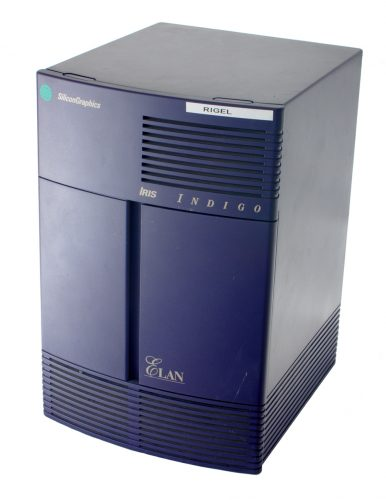
\includegraphics[scale=0.3]{HRmYIY.png}
		\centering
		\caption{SGI Indigo. Disponível em: \newline 				$http://image.jeuxvideo.com/medias-sm/149393/1493928395-8148-capture-d-ecran.jpg$}
	\end{figure}
	\item Sony Playstation 2: O PlayStation 2 (oficialmente abreviado como PS2) foi o segundo console produzido pela empresa Sony, após o PlayStation original. Foi lançado no dia 4 de março de 2000 no Japão, no dia 26 de outubro na América do Norte, e posteriormente, no dia 24 de novembro na Europa. Após um lento primeiro ano, o PlayStation 2 cresceu a ponto de tornar-se o console mais vendido da história dos videogames, ele possui processador MIPS III R5900
		\begin{figure}[H]
		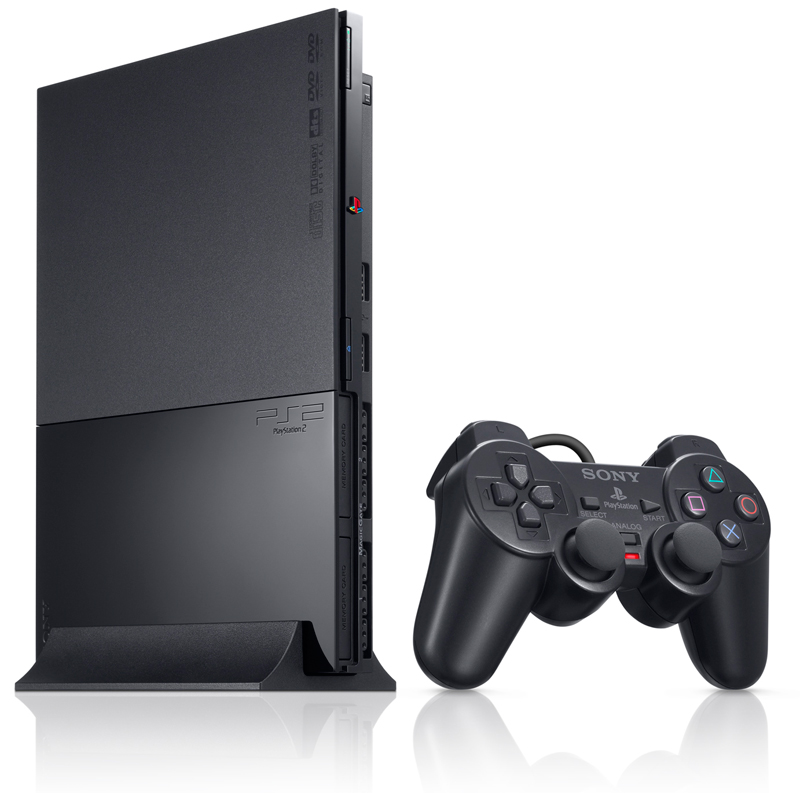
\includegraphics[scale=0.3]{CxvmeX.png}
		\centering
		\caption{Sony Playstation 2. Disponível em: \newline 								$	https://vn-live-02.slatic.net/p/2/may-playstation-2-sony-slim-den-1480682719-8470201-d27a35baa637d81d533ef18f36465270.jpg$}
	\end{figure}

	\item Nintendo 64 (MIPS R4300i CPU): O primeiro grande console de 64 bits foi lançado em 1996 e roda com  93,75 MHz
	\begin{figure}[H]
		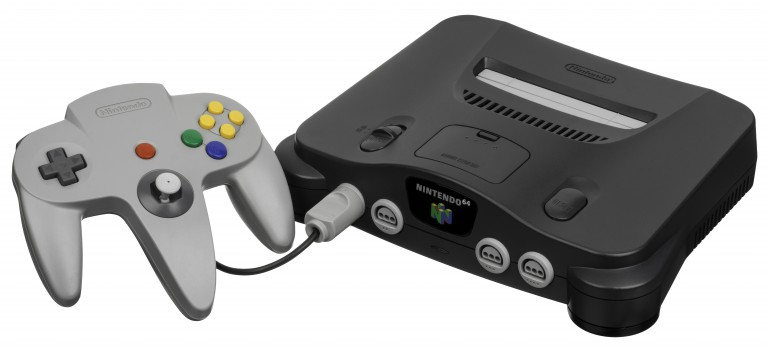
\includegraphics[scale=0.3]{ft4vaB.png}
		\centering
		\caption{Nintendo 64. Disponível em: \newline 								$http://www.pelimies.fi/media/catalog/product/cache/1/image/ \newline 9df78eab33525d08d6e5fb8d27136e95/n/i/nintendo-64-wcontroller-l.jpg$}
	\end{figure}

	\item Tesla S: O Model S, esportivo elétrico da montadora de Elon Musk, tem preços de tabela entre R$ 745 mil e R$ 785 mil e utiliza uma CPU MIPS I
	\begin{figure}[H]
		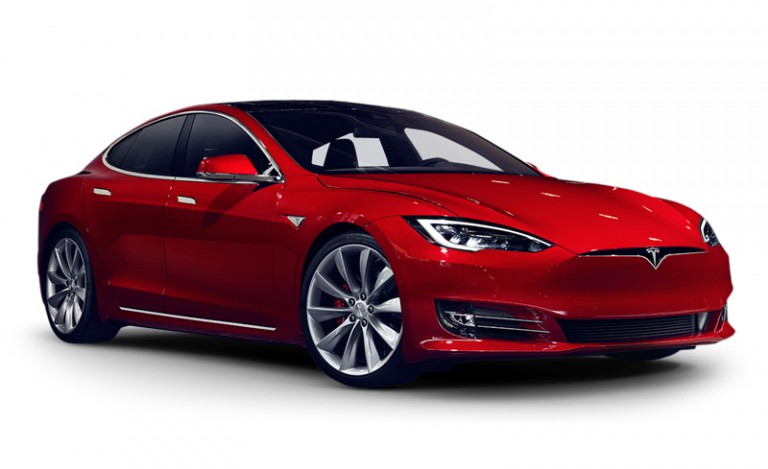
\includegraphics[scale=0.3]{xna8fZ.png}
		\centering
		\caption{Tesla S. Disponível em: $https://\newline d3egew7zjohdb1.cloudfront.net/incoming/jeyezn-Tesla1.jpg/ \newline ALTERNATES/LANDSCAPE_1140/Tesla1.jpg$}
	\end{figure}
	

\end{itemize}
\section*{Referências Bibliográficas}
\bibliographystyle{plain}
\bibliography{bibliografia}

\end{document}